El filtro Halftone parte a la imagen original en bloques de 2x2 píxeles, se obtiene t como la sumatoria del valor de cada pixel y genera un bloque del mismo tamaño en la imagen destino que cumpla:

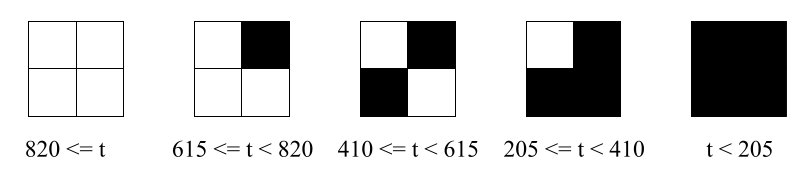
\includegraphics[width=\textwidth]{halftone1.jpg} 

\begin{itemize}
\item El pixel de arriba a la izquierda es blanco si $t \geq$ 205.
\item El pixel de arriba a la derecha es blanco si $t \geq$ 820.
\item El pixel de abajo a la izquierda es blanco si $t \geq$ 615.
\item El pixel de abajo a la derecha es blanco si $t \geq$ 410.
\end{itemize}

Si el ancho y/o alto de la imagen es impar, se descarta la última fila y/o columna, según corresponda.

\subsubsection{Implementación en C}

Con dos ciclos anidados se recorre de 2 en 2 la imagen original.
Se calcula t con la suma de de los valores de los 4 píxeles y luego se setean los píxeles en blanco o negro según corresponda por el valor de $t$.

\subsubsection{Implementación en Assembler}

También se realizan dos ciclos anidados, trayendo cada vez de a 32 píxeles.
Se traen 16 píxeles de la primera línea a xmm0 y 16 de la segunda línea a xmm1.
Como para calcular $t$ se necesita un espacio de más de 1 byte ($t$ puede ser mayor a 255), se desempaquetan y se trabaja primero con los 8 bytes menos significativos, guardando el resto para procesar al terminar estos.
Se suman los 2 registros verticalmente, luego se shiftea un registro para acomodar y volver a sumar.
Esto da como resultado el valor $t$ para cada uno de los 4 bloques como se ve en la siguiente ilustración:

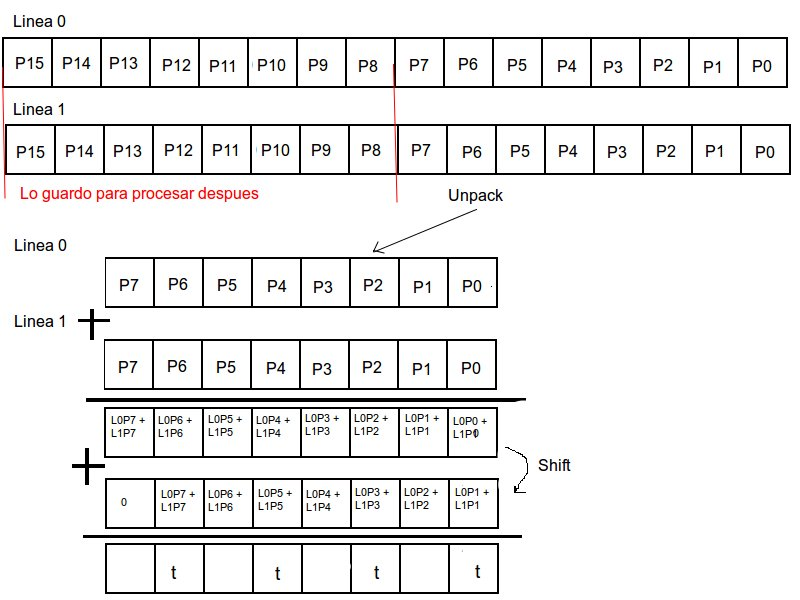
\includegraphics[width=\textwidth]{halftone2.jpg} 

Se compara por mayor o igual en un registro distinto para cada uno de los valores límite.
Luego, ya que  el valor que va a cada pixel es el mismo que el resultado de la comparación (todos 1s o todos 0s), simplemente se ordenan los resultados en los primeros 8 bytes de cada registro.
Se ilustra el proceso para los bytes de la primera línea:

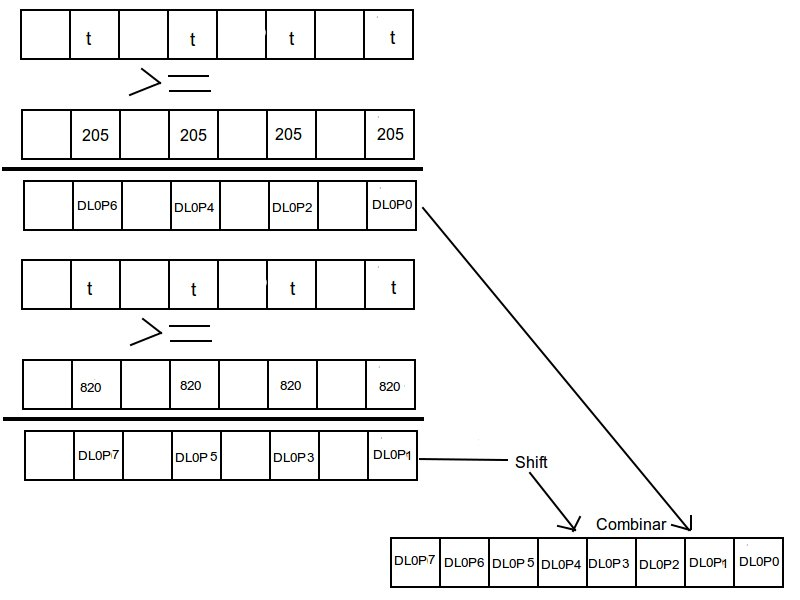
\includegraphics[width=\textwidth]{halftone3.jpg} 

Este proceso se repite con los 8 bytes más significativos que guardamos al principio. Estos resultados se shiftean 8 bytes a la izquieda y combinan (con un $por$) con los primeros resultados, dándonos 2 registros con 16 bytes procesados cada uno, que se copian a la memoria de la imagen destino.

En el caso que el ancho no sea múltiplo de 16, antes de entrar al ciclo se calcula el resto ($width$ \% 16) y en la primera iteración de cada fila se suma este resto en lugar de los 16 que se suman normalmente.

\subsubsection{Resultados}

En la implementación en C, para procesar un bloque de 4 píxeles se requieren 8 accesos a memoria (4 lecturas y 4 escrituras), en cambio en la implementación en ASM, se procesa un bloque de 32 píxeles con tan sólo 4 accesos a memoria.
Con esos datos y, teniendo en cuenta que el acceso a memoria es mucho más lento que cualquier otra operación que se aplique en el filtro, la implementación en ASM debería ser aproximadamente 16 veces más rápida que la implementación en C.

Ejecutamos ambos filtros 1000 veces cada uno y estos son los resultados obtenidos:

\begin{center}
    \begin{tabular}{|l|l|l|}
        \hline
         & Implementación C & Implementación en asm  \\
        \hline
        Duración promedio (en ciclos de clock) & 3 229 822       & 230 612                 \\
        \hline
    \end{tabular}
\end{center}

Como se puede observar, la implentación en asm es $\sim$14 veces más rápida, lo que corrobora nuestra hipótesis.
